%Validation_OhmsLaw
\chapter{Validation of Ohm's Law}
\vspace{-0.25in}
What physicists do is to try to understand how the universe works. To do this we use the Scientific Method. And what makes the scientific method different from philosophy is the use of experimentation to verify our ideas.

So in a physics lab class, we need to test ideas about how the universe works. We call these ideas ``mental models'' or just ``models.'' We have been using one of these models in making voltage measuring devices already. It was called Ohm's law. Let's start out by testing Ohm's law to see if it really works.

\section{Ohm's Law Revisited}

We learned several labs ago that voltage and current are linearly related to each other. This is what we would call a \emph{model}, a mental understanding of how part of the universe works. Usually in physics we distill the model into an equation. We call this equation a law. In this case, Ohm's law. 

\begin{equation*}
	\Delta V=IR
\end{equation*}

\noindent where $R$ is the slope of the $\Delta V$ vs. $I$ curve. We can see the model relationship between $\Delta V$ and $I$ reflected in the equation. Note that being a ``law'' doesn't mean the equation is always true. The word ``law'' generally implies that the equation is true at least some of the time, but really it is telling us we have distilled our model into math.

We might plot our equation to show the $\Delta V$ vs. $I$ relationship.

\begin{figure}[h!]
	\centering
	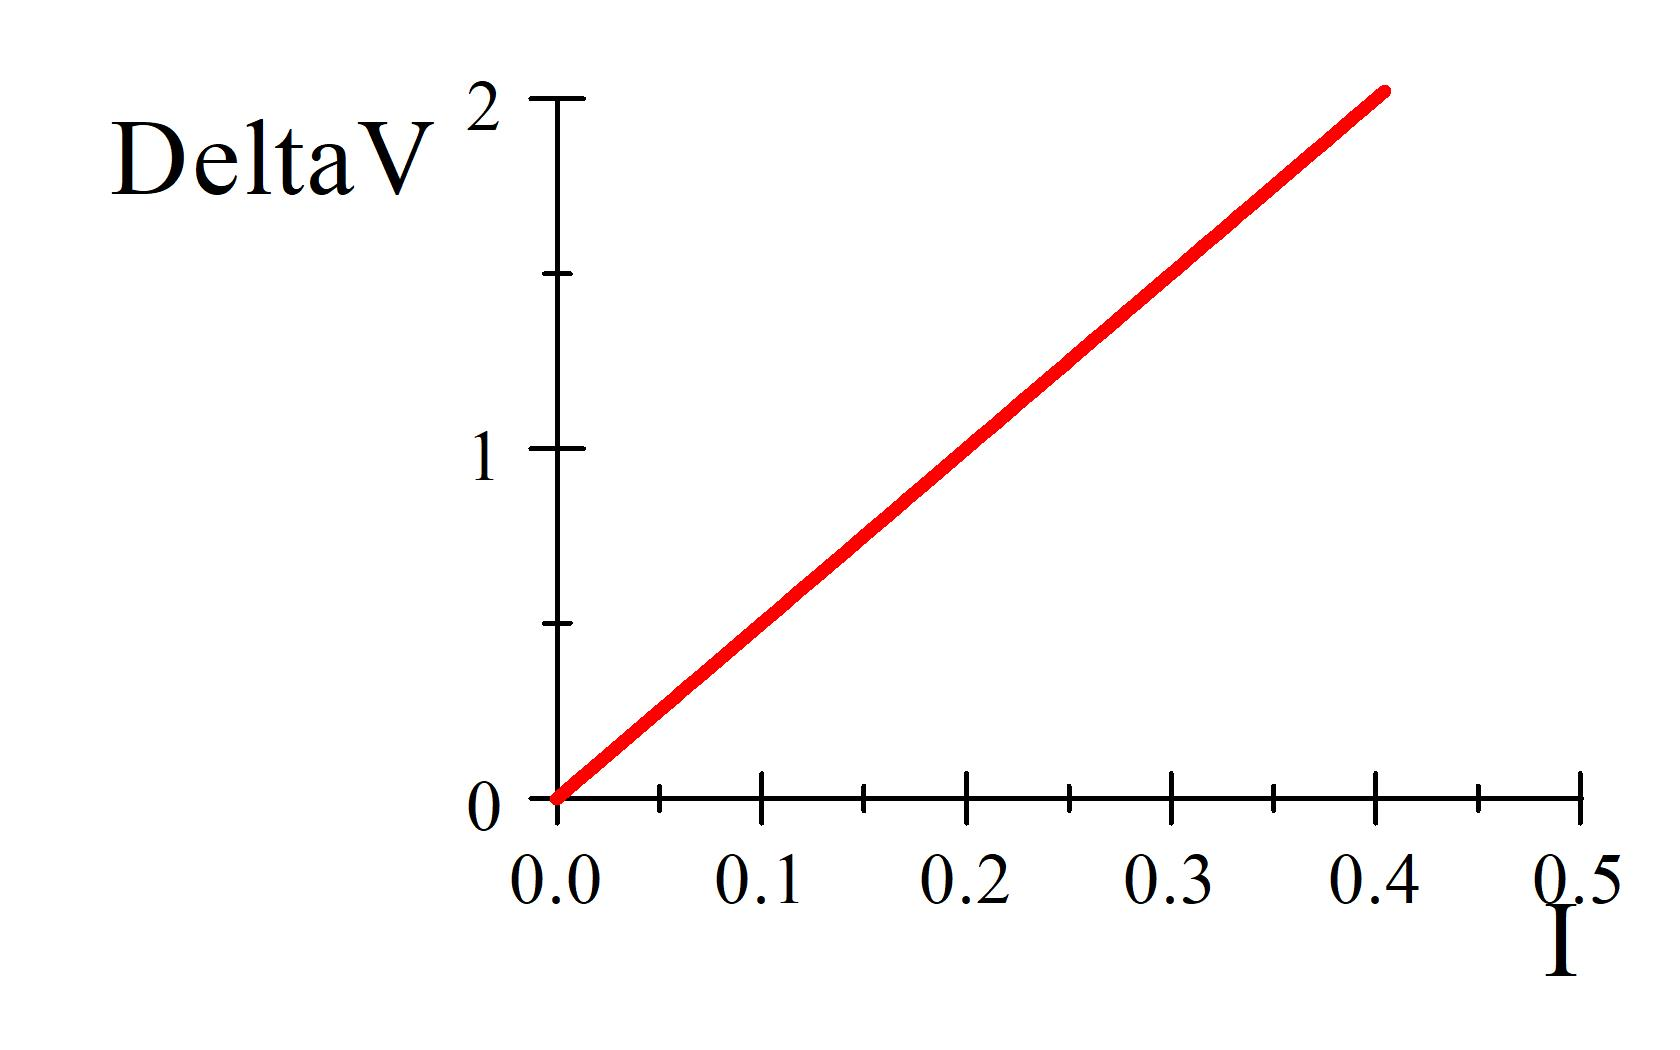
\includegraphics[width=2.0in,height=1.4in]{PH4CAV2O}
\end{figure}



\noindent But as scientists, we should ask, does our model work for all materials? What if we graphed $\Delta V$ vs $I$ for some device and found a graph that looks like this?

\begin{figure}[h!]
	\centering
	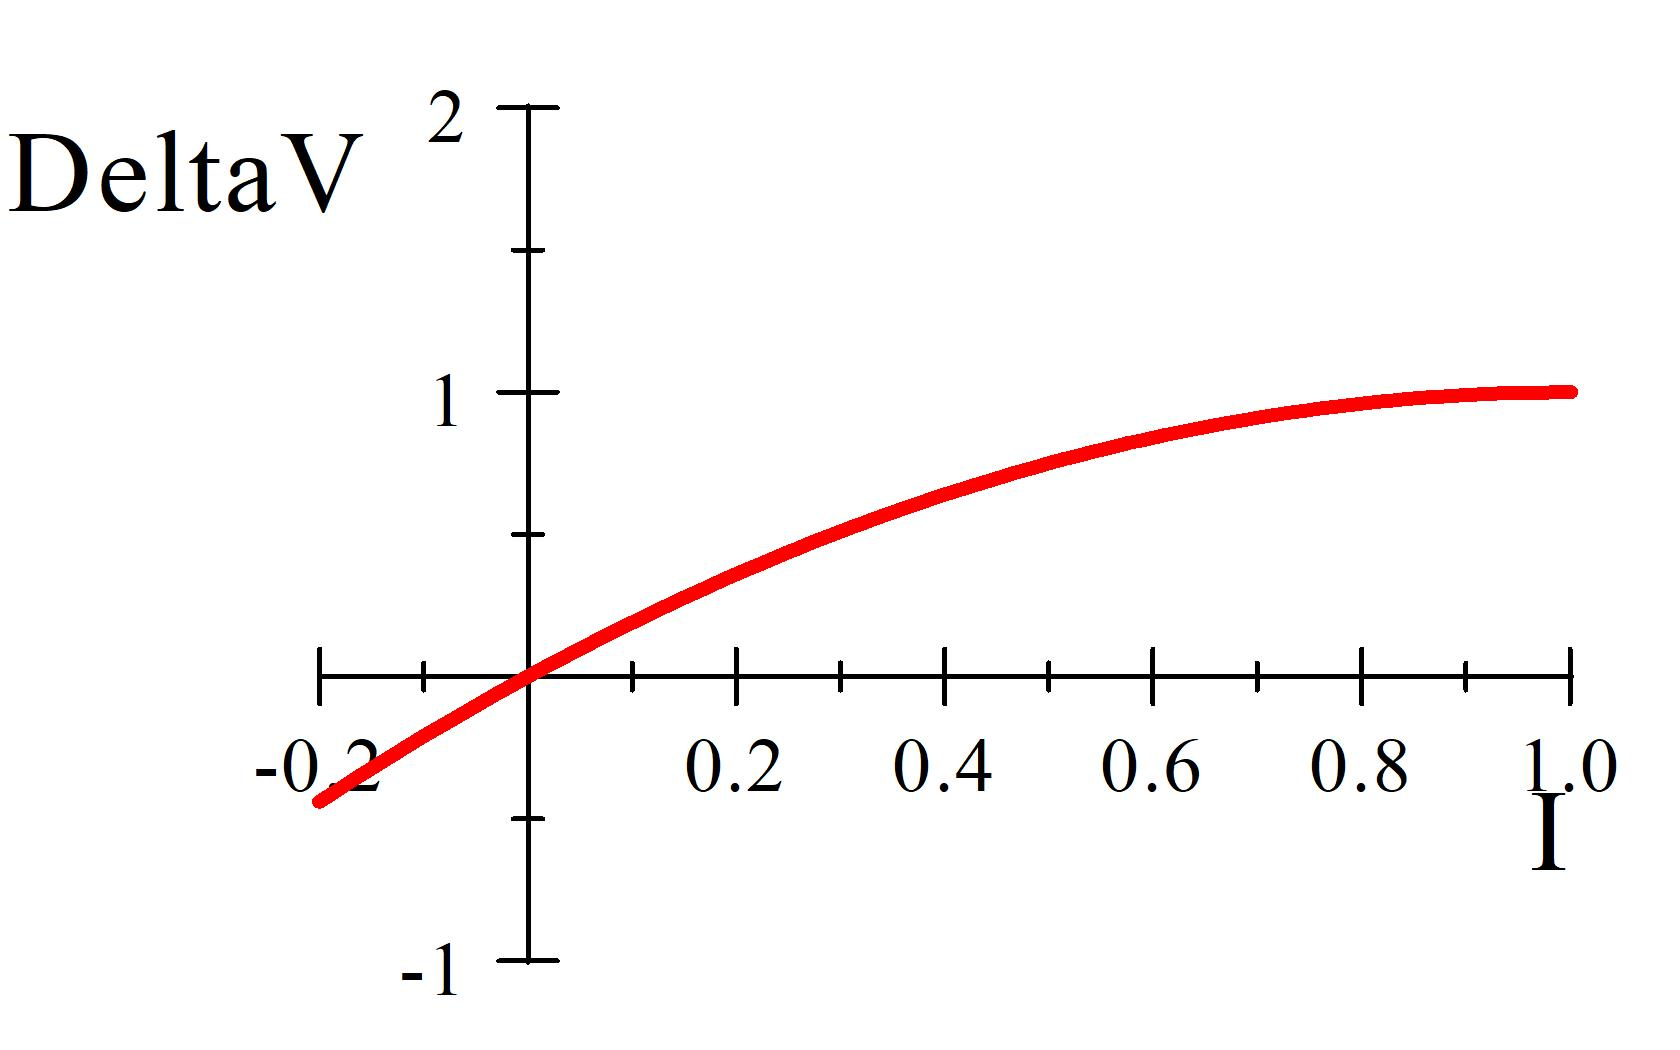
\includegraphics[width=2.2606in,height=1.5177in]{PH4CAV2P}
\end{figure}

\noindent Such a device would \emph{not} follow Ohm's law. We would say that such a device is \emph{nonohmic}.

Today we will test our model by taking $\Delta V$ and $I\ $measurements and seeing if the equation $\Delta V=IR$ describes the data well. Of course, this means we need to measure two things at once with our Arduino. We need both $\Delta V$ and $I.$ But this isn't a problem because our Arduninos have five analog inputs. So we just need to have one measurement attached to, say, pin A0 and another to, say, pin A1. Of course both will need to be
connected to GND as the second measurement because $\Delta V$ measurements
take two leads. 

But wait, if we are testing Ohm's law, we don't want two $\Delta V$ measurements, we want $\Delta V$ and $I.$ How do we get $I$ measured by an Arduino?

\subsection{Measuring current with our Arduino}

Arduinos and other DAQs only measure voltages. Let's review how we measure the voltage across a resistor, and then review how to turn that voltage measurement into a current measurement.

\begin{figure}[h!]
	\centering
	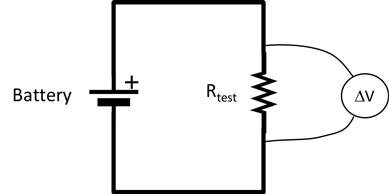
\includegraphics[width=3.2785in,height=1.6449in]{PH4CAV2Q}
\end{figure}

We put the two leads of a voltmeter (shown as a circle with a $\Delta V$\ in it) on either side of the resistor that we are testing. If the voltmeter is our Arduino, the leads on the side of the resister connected to the positive side of the battery should go to A0 and the lead connected to the negative side of the battery should be connected to GND. This is all what an Arduino (or any other DAQ) can do.

To measure a current with our Arduino we have to somehow turn that current into a voltage. This is true of most measurements we will do. We need to turn temperature, or humidity, or magnetic field, or light intensity into a voltage. Turning magnetic field into a voltage is a little tricky, but we already know all we need to know to handle current.

To turn a current into a voltage, think of Ohm's law again.

\begin{equation*}
	\Delta V_{s}=IR_{s}
\end{equation*}

\noindent we can solve for $I$

\begin{equation*}
	I=\frac{\Delta V_{s}}{R_{s}}
\end{equation*}

\noindent so if we add a new resistor, $R_{s}$ to the circuit,

\begin{figure}[h!]
	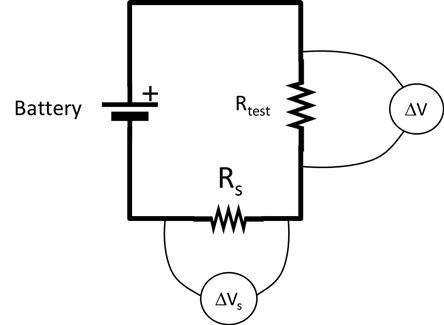
\includegraphics[width=3.7395in,height=2.7423in]{PH4CAV2R}
\end{figure}

\noindent and measure the voltage across that circuit, we will be able to calculate the current. This is familiar from an earlier lab. We called this extra resistor a ``shunt'' resistor.

Of course, if $R_{s}$ is very large, then $R_{s},$ itself, will slow down the current. So we want to choose a $R_{s}$ that is much less than $R_{test}. $

\begin{equation*}
	R_{s}\ll R_{test}
\end{equation*}

\noindent But so long as this is true, our $R_{s}$ won't change the current much, and since we know $R_{s}$ we know the current 

\begin{equation*}
	I=\frac{\Delta V_{s}}{R_{s}}
\end{equation*}

\noindent We have turned our current measurement into a voltage measurement!

\subsection{Actually making an Arduino measure current}

This idea is great, but let's talk a little bit about how to wire this dual measurement. Think again about our two voltage measurements, $\Delta V$ and $\Delta V_{s}.$ Each $\Delta $ implies two measurements. That means we need a total of four measurements to make this work! Let's see where these measurements would be on our circuit diagram.

\begin{figure}[h!]
	\centering
	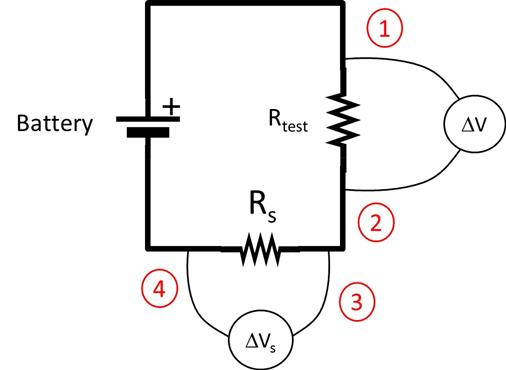
\includegraphics[width=3.2583in,height=2.1185in]{PH4CAV2S}
\end{figure}

By drawing the diagram, we realize that we can create both $\Delta V$ measurements with only three individual voltage measurements because the voltage at point 2 and the voltage at point 3 should be the same. So we could wire our circuit like this:

\begin{figure}[h!]
		\centering
	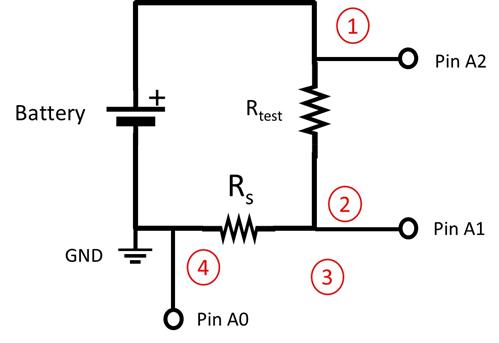
\includegraphics[width=3.2583in,height=2.1185in]{PH4CAV2T}
\end{figure}

\noindent and of course we need to wire the negative pole of the battery or power supply to the GND pin. Then our two voltage difference measurements will be formed from 

\begin{eqnarray*}
	\Delta V &=&V_{A2}-V_{A1} \\
	\Delta V_{s} &=&V_{A1}-V_{A0}
\end{eqnarray*}

If we keep our voltage from our battery or power supply in the $0\unit{V}$ to $+5\unit{V}$ range, then we can use our simple voltmeter sketch. We do need to modify it to take three different voltage measurements. And we need to add the math to make $\Delta V_{s}$ into $I.$ We could even modify this so that our code would report out 

\begin{equation*}
	R=\frac{\Delta V}{I}
\end{equation*}

\noindent and we might as well. Here is an example sketch.

%%%%%%%%%%%%%%%%%%%%%%%%%%%%%%%%%%%%%%%%%%%%%%%%%%%%%%%%%%%%%%%%%%%%%%%%
% code link here for download
%\href{https://dtoliphant.github.io/PH250Manual/Code/OhmsLaw_SimpleVA.ino}{Download here}
%\href{https://dtoliphant.github.io/PH250Manual/Code/DAQ_Extended_voltmeter.ino}{Download here}
\href{https://raw.githubusercontent.com/rtlines/IntermediateLabPH250/main/Code/OhmsLaw_SimpleVA.ino}{Download here}
%%%%%%%%%%%%%%%%%%%%%%%%%%%%%%%%%%%%%%%%%%%%%%%%%%%%%%%%%%%%%%%%%%%%%%%%
\lstinputlisting[language=Arduino]{Code/OhmsLaw_SimpleVA.ino}

\subsubsection{Choosing shunt resistors}

It's harder than you might think to choose a good shunt resistor. The shunt resistor resistance shouldn't be big enough to cause too much error in our $\Delta V$ measurement for the resistor we want to measure (Think of our voltage divider, the two resistors will share the voltage from the battery, so every bit of $\Delta V_{shunt}$ is error in our measurement of $\Delta V_{test}$).

The shunt resistance should also be small enough that it doesn't effect the current much. But suppose we find the smallest resistor that we can, say, $10\unit{\Omega}.$ Surely that will not affect the actual $\Delta V$ or $I$ measurements. But still, we may have a problem. Let's consider an actual circuit to see why.

Suppose we have a circuit where the input voltage from the power supply is $\Delta V_{ps}=2\unit{V}$ and our test resistor is $R=5000\unit{\Omega}.$ And suppose we try to use $R_{s}=10\unit{\Omega}.$ 

\begin{figure}[h!]
	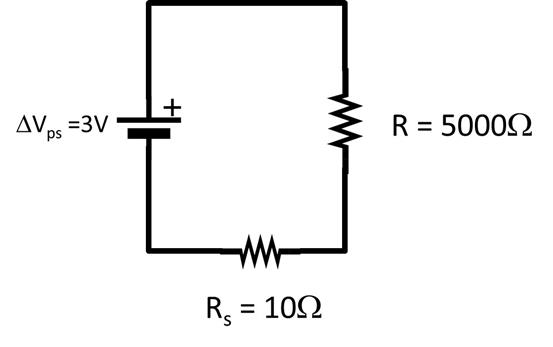
\includegraphics[width=4.6527in,height=2.9265in]{PH4CAV2U}
\end{figure}

The two resistors together are a voltage divider. So we expect the voltage drop across each resistor to sum to the voltage given by the power supply

\begin{equation*}
	\Delta V_{ps}=\Delta V_{R}+\Delta V_{s}
\end{equation*}

\noindent and we know the current will be the same in the entire circuit. We can use Ohm's law to find the current.

\begin{equation*}
	\Delta V_{ps}=IR_{total}
\end{equation*}

\noindent so that 

\begin{eqnarray*}
	I &=&\frac{\Delta V_{ps}}{R_{total}} \\
	  &=&\frac{\Delta V_{ps}}{R+R_{s}}
\end{eqnarray*}

Now we can find the voltage drop across just $R_{s}$

\begin{eqnarray*}
	\Delta V_{s} &=&IR_{s} \\
                 &=&\left( \frac{\Delta V_{ps}}{R+R_{s}}\right) R_{s}
\end{eqnarray*}

\noindent and let's put in numbers

\begin{eqnarray*}
	\Delta V_{s} &=&\left(\frac{2\unit{V}}{5000\unit{\Omega}+10\unit{\Omega}}\right) \left( 10\unit{\Omega}\right) \\
    &=&3.\,\allowbreak 992\times 10^{-3}\unit{V} \\
    &=&3.\,\allowbreak 992\unit{mV}
\end{eqnarray*}

\noindent Remember that for our simple voltmeter, 

\begin{equation*}
	\Delta V_{\min }=\frac{5\unit{V}}{1024}=4.\,\allowbreak 88\unit{mV}
\end{equation*}

\noindent and this is larger than $\Delta V_{s}$ so once we use our Arduino analog to digital converter $\Delta V_{s}$ will appear to be zero! Our current meter that we built will say our current measurement will be zero even thought there is a current flowing. That is a 100\% error!

We might try to improve things by increasing the power supply voltage. Even
if we increased the voltage from the power supply to, say, $5\unit{V}$ (our
maximum) we would only have 

\begin{eqnarray*}
	\Delta V_{s}   &=&\left(\frac{5\unit{V}}{5000\unit{\Omega}+10\unit{\Omega}}\right) \left( 10\unit{\Omega}\right) \\
    &=&9\,.98\unit{mV}
\end{eqnarray*}

We should compare this value to our ADC minimum detectable value 

\begin{equation*}
	\frac{\Delta V_{s}}{\Delta V_{\min }}=N
\end{equation*}

\noindent the number of ADC units that will be used. We can see that for $R_{s}=10\unit{\Omega}$ 

\begin{equation*}
	N=\frac{9\,.98\unit{mV}}{4.\,\allowbreak 88\unit{mV}}=2
\end{equation*}

\noindent ADC units. With our entire value of $\Delta V_{s}$ split into only two numbers our uncertainty in our $\Delta V_{s}$ would be something like $50\%.$ That won't make a very good current measurement.

Suppose instead, we use $R_{s}=170\unit{\Omega}.$  This is much bigger, so it will affect the voltage measurement of the test resistor a little. But in the end will work better. If we set our power supply back to $\Delta V_{ps}=2\unit{V}$ the $R_{s}=170\unit{\Omega}$ gives. 

\begin{eqnarray*}
	\Delta V_{s} &=&\left( \frac{2\unit{V}}{5000\unit{\Omega}+170\unit{\Omega}}\right) \left( 170\unit{\Omega}\right) \\
                 &=&65.\,\allowbreak 764\unit{mV}
\end{eqnarray*}

\noindent This would give 

\begin{equation*}
	N=\frac{65.\,\allowbreak 764\unit{mV}}{4.\,\allowbreak 88\unit{mV}}=13.\,\allowbreak 476
\end{equation*}

\noindent or about $13$ ADC units spread across our $65.\,\allowbreak 764\unit{mV}.$ Then each of our ADC units would be worth 

\begin{equation*}
	\delta \Delta V_{s}=\frac{65.\,\allowbreak 764\unit{mV}}{13}=5.\,\allowbreak1\unit{mV}
\end{equation*}

This is very near the $\Delta V_{\min }=$ $4.88\,\allowbreak \unit{mV}$ value, but a little bit higher. If $\delta \Delta V_{s}$ from our calculation is larger than $\delta V_{\min ,}$ then we have to use the larger value as our uncertainty in $\Delta V_{s}.$ So we would say $\delta \Delta V_{s}=5.\,\allowbreak 1\unit{mV}.$ But still this is not a terrible error.  Now our percent error is
\begin{equation*}
	100\times \frac{5.\,\allowbreak 058\,8\unit{mV}}{65.\,\allowbreak 764\unit{mV}}=7.\,\allowbreak 7\%
\end{equation*}

\noindent which is much better than $50\%$ or $100\%$ error. You might guess that we can do a little better by trying other resistance values. And you would be right. But if you only need an $8\%$ error, this value would be fine.

Our stand-alone meters have lots of shunt resistors inside of them. You are changing shunt resistors when you change the dial setting, trying to balance these errors. By changing shunt resistors in our circuit we are doing the same thing as turning the dial on the current settings of a multimeter.

\subsection{Finding Uncertainty in a calculated value}

In the last section I\ gave errors in $\Delta V_{s},$ but didn't finish the error in the current, $I.$ Of course, since we had to calculate the current, we also need to find the uncertainty in our current using error propagation. Fortunately we ``remember'' how to do this from PH150. We use our basic form for standard error propagation. If we have a function $f\left( x,y,z\right) $ then the uncertainty in $f$ would be 

\begin{equation*}
	\delta f=\sqrt{\left( \left( \frac{\partial f}{\partial x}\right)\left(\delta x\right) \right) ^{2}+\left( \left( \frac{\partial f}{\partial y}\right) \left( \delta y\right) \right) ^{2}+\left( \left( \frac{\partial f}{\partial z}\right) \left( \delta z\right) \right) ^{2}}
\end{equation*}

In our current case, our function $f$ is the current $I$ and it is a function of $\Delta V_{s}$ and $R_{s}$ 

\begin{equation*}
	f=I=\frac{\Delta V_{s}}{R_{s}}
\end{equation*}

\noindent so we will have an uncertainty like this

\begin{equation*}
	\delta I=\sqrt{\left( \left( \frac{\partial I}{\partial \Delta V_{s}}\right) \left( \delta \Delta V_{s}\right) \right) ^{2}+\left( \left( \frac{\partial I}{\partial R_{s}}\right) \left( \delta R_{s}\right) \right) ^{2}}
\end{equation*}

\noindent and we can find the partial derivatives

\begin{equation*}
	\frac{\partial I}{\partial \Delta V_{s}}=\frac{1}{R_{s}}
\end{equation*}

\begin{equation*}
	\frac{\partial I}{\partial R_{s}}=-\frac{\Delta V_{s}}{R_{s}^{2}}
\end{equation*}

\noindent so we have 

\begin{equation*}
	\delta I=\sqrt{\left( \left( \frac{1}{R_{s}}\right) \left( \delta \Delta V_{s}\right) \right) ^{2}+\left( \left( -\frac{\Delta V_{s}}{R_{s}^{2}}\right) \left( \delta R_{s}\right) \right) ^{2}}
\end{equation*}

Let's try this for our example in the last section. We have $R_{s}=170\unit{\Omega}.$ We know that $\delta \Delta V_{s}=$ $5.\,\allowbreak 058\,8\unit{mV}$ and our resistors are only good to $1\%$ so that would be $\delta R_{S}=1.7\unit{\Omega}$

\begin{eqnarray*}
	\delta I &=&\sqrt{\left( \left( \frac{1}{170\unit{\Omega}}\right) \left( 5.\,\allowbreak 058\,8\unit{mV}\right) \right) ^{2}+\left(
	\left( -\frac{65.\,\allowbreak 764\unit{mV}}{\left( 170\unit{\Omega}\right) ^{2}}\right) \left( 1.7\unit{\Omega}\right) \right) ^{2}} \\
            &=&3.\,\allowbreak 000\,8\times 10^{-5}\unit{A}
\end{eqnarray*}

This looks small. Is it a good uncertainty? We can't tell until we compare
it to our expected current. We expect for our example 

\begin{eqnarray*}
	I &=&\frac{\Delta V_{ps}}{R} \\
	  &=&\frac{2\unit{V}}{5000\unit{\Omega}} \\
      &=&\allowbreak 0.000\,4\unit{A} \\
      &=&4\times 10^{-4}\unit{A}
\end{eqnarray*}

\noindent so the fractional uncertainty in the current will be 

\begin{equation*}
	100\frac{3.\,\allowbreak 000\,8\times 10^{-5}\unit{A}}{4\times 10^{4}\unit{A}}=7.\,\allowbreak 502\
\end{equation*}


This still isn't great, it's about what we got for the error in $\delta \Delta V_{s}$ (but it's better than $50\%$). We might be able to do better. But if $8\%$ is OK for our application, then we stop here!

Let's try to figure out what the biggest contributor to our uncertainty might be. To do this we look at the terms in our uncertainty calculation separately

\begin{eqnarray*}
	\left( \left( \frac{1}{R_{s}}\right) \left( \delta \Delta V_{s}\right)\right) ^{2} &=&\left( \left( \frac{1}{170\unit{\Omega}}\right) \left( 5.\,\allowbreak 058\,8\unit{mV}\right) \right) ^{2}=\allowbreak 8.\,\allowbreak 855\,2\times 10^{-10}\unit{A}^{2} \\
	\left( \left( -\frac{\Delta V_{s}}{R_{s}^{2}}\right) \left( \delta R_{s}\right) \right) ^{2} &=&\left( \left( -\frac{65.\,\allowbreak 764\unit{mV}}{\left( 170\unit{\Omega}\right) ^{2}}\right) \left( 1.7\unit{\Omega}.\right) \right) ^{2}=\allowbreak 1.\,\allowbreak 496\,5\times 10^{-11}%\unit{A}^{2}
\end{eqnarray*}

The first term is about sixty times the second. So to make an improvement we would want to first concentrate on the first term. We could change our $\delta \Delta V_{s}$ or change our $R_{s}$ value. Changing $\Delta V_{s}$ is harder than changing $R_{s}.$ Maybe we could even make $R_{s}$ a little
bigger to improve our current measurement. \emph{Notice that this was not
the obvious solution!} At first it seemed that smaller $R_{s}$ values would
give better uncertainties. But after doing the uncertainty calculations, we
find that there is an optimal range for $R_{s}.$ Big $R_{s}$ is still bad,
but very small $R_{s}$ is also bad. You have to do the math to find this out.

\subsubsection{Iterate to find an optimal value}

Since there is an $R_{s}$ in the bottom of both terms in our current uncertainty, let's try changing the $R_{s}$ value and see if the uncertainty gets better. We have to start all the way back at the top with $\Delta V_{s}. $ We will have to go through all our calculations again! A symbolic math processor or python might be a good way to go so you aren't putting the same things in your calculator over and over.

We start by finding the current in the circuit

\begin{equation*}
	I=\left( \frac{\Delta V_{ps}}{R+R_{s}}\right)
\end{equation*}

\noindent Then an estimate for $\Delta V_{s}$ across the shunt resistor would be

\begin{eqnarray*}
	\Delta V_{s} &=&IR_{s} \\ &=&\left( \frac{\Delta V_{ps}}{R+R_{s}}\right) R_{s}
\end{eqnarray*}

\noindent and then the number of ADC units we used will be 

\begin{equation*}
	N_{ADC}=\frac{\Delta V_{s}}{\Delta V_{\min }}
\end{equation*}

\noindent rounded to the smallest integer, which gives a new estimate of our uncertainty in $\Delta V_{s}$ 

\begin{equation*}
	\delta \Delta V_{s}=\frac{\Delta V_{s}}{N_{ADC}}
\end{equation*}

\noindent and now we need can find the uncertainty in $I$

\begin{equation*}
	\delta I=\sqrt{\left( \left( \frac{1}{R_{s}}\right) \left( \delta \Delta V_{s}\right) \right) ^{2}+\left( \left( -\frac{\Delta V_{s}}{R_{s}^{2}} \right) \left( \delta R_{s}\right) \right) ^{2}}
\end{equation*}

\noindent and its fractional uncertainty

\begin{equation*}
	f_{I}=\frac{\delta I}{I}
\end{equation*}

As you can see, it is probably best to put all this in a symbolic package (like Mathmatica or Maple, or Sage, or python's sympy, or whatever your favorite symbolic math processor might be). That way, you can change values of, say, $R_{s}$ and $\Delta V_{s}$ without redoing everything. At least consider using a spreadsheet program or even in Python!.

Let's try this once more with $R_{s}=500\unit{\Omega}$ just to see what would happen.

\begin{eqnarray*}
	I &=&\left( \frac{2\unit{V}}{5000\unit{\Omega}+500\unit{\Omega}}\right) \\
      &=&3.\,\allowbreak 636\,4\times 10^{-4}\unit{A}
\end{eqnarray*}

\noindent so

\begin{eqnarray*}
	\Delta V_{s} &=&IR_{s} \\
                 &=&\left( \frac{2\unit{V}}{5000\unit{\Omega}+500\unit{\Omega}}\right) \left( 500\unit{\Omega}\right) \\
                 &=&0.181\,82\unit{V}
\end{eqnarray*}

\noindent and then the number of ADC units we used will be 

\begin{equation*}
     N_{ADC}=\frac{0.181\,82\unit{V}}{4.\,\allowbreak 88\unit{mV}}=37.\,\allowbreak 258
\end{equation*}

\noindent which gives a new estimate of our uncertainty in $\Delta V_{s}$ 

\begin{equation*}
    \delta \Delta V_{s}=\frac{0.181\,82\unit{V}}{37}=4.\,\allowbreak914\,1\times 10^{-3}\unit{V}
\end{equation*}

\noindent and now we need can find the uncertainty in $I.$ We will need $\delta
R_{s}=500\unit{\Omega}\times 0.01=\allowbreak 5.0\unit{\Omega}$

\begin{equation*}
	\delta I=\sqrt{\left( \left( \frac{1}{500\unit{\Omega}}\right) \left( \delta \Delta V_{s}\right) \right) ^{2}+\left( \left( -\frac{\Delta V_{s}}{\left( 500\unit{\Omega}\right) ^{2}}\right) \left( \delta R_{s}\right) \right) ^{2}}
\end{equation*}

\begin{eqnarray*}
	\delta I &=&\sqrt{\left( \left( \frac{1}{500\unit{\Omega}}\right) \left( 4.\,\allowbreak 914\,1\times 10^{-3}\unit{V}\right) \right)^{2}+\left( \left( -\frac{0.181\,82\unit{V}}{\left( 500\unit{\Omega}\right) ^{2}}\right) \left( 5.0\unit{\Omega}\right) \right) ^{2}} \\
            &=&1.\,\allowbreak 047\,9\times 10^{-5}\unit{A}
\end{eqnarray*}

\noindent and its fractional uncertainty

\begin{equation*}
	f_{I}=100\times \frac{1.\,\allowbreak 047\,9\times 10^{-5}\unit{A}}{3.\,\allowbreak 636\,4\times 10^{-4}\unit{A}}=2.\,\allowbreak 881\,7\
\end{equation*}


This was a bit of an improvement! We could continue to iterate. I had my
computer do this for $R=5000\unit{\Omega}$ and $\Delta V_{ps}=2\unit{V}$ I asked it to plot $f_{I}$ as a function of $R_{s}$ 

\begin{figure}[h!]
	\centering
	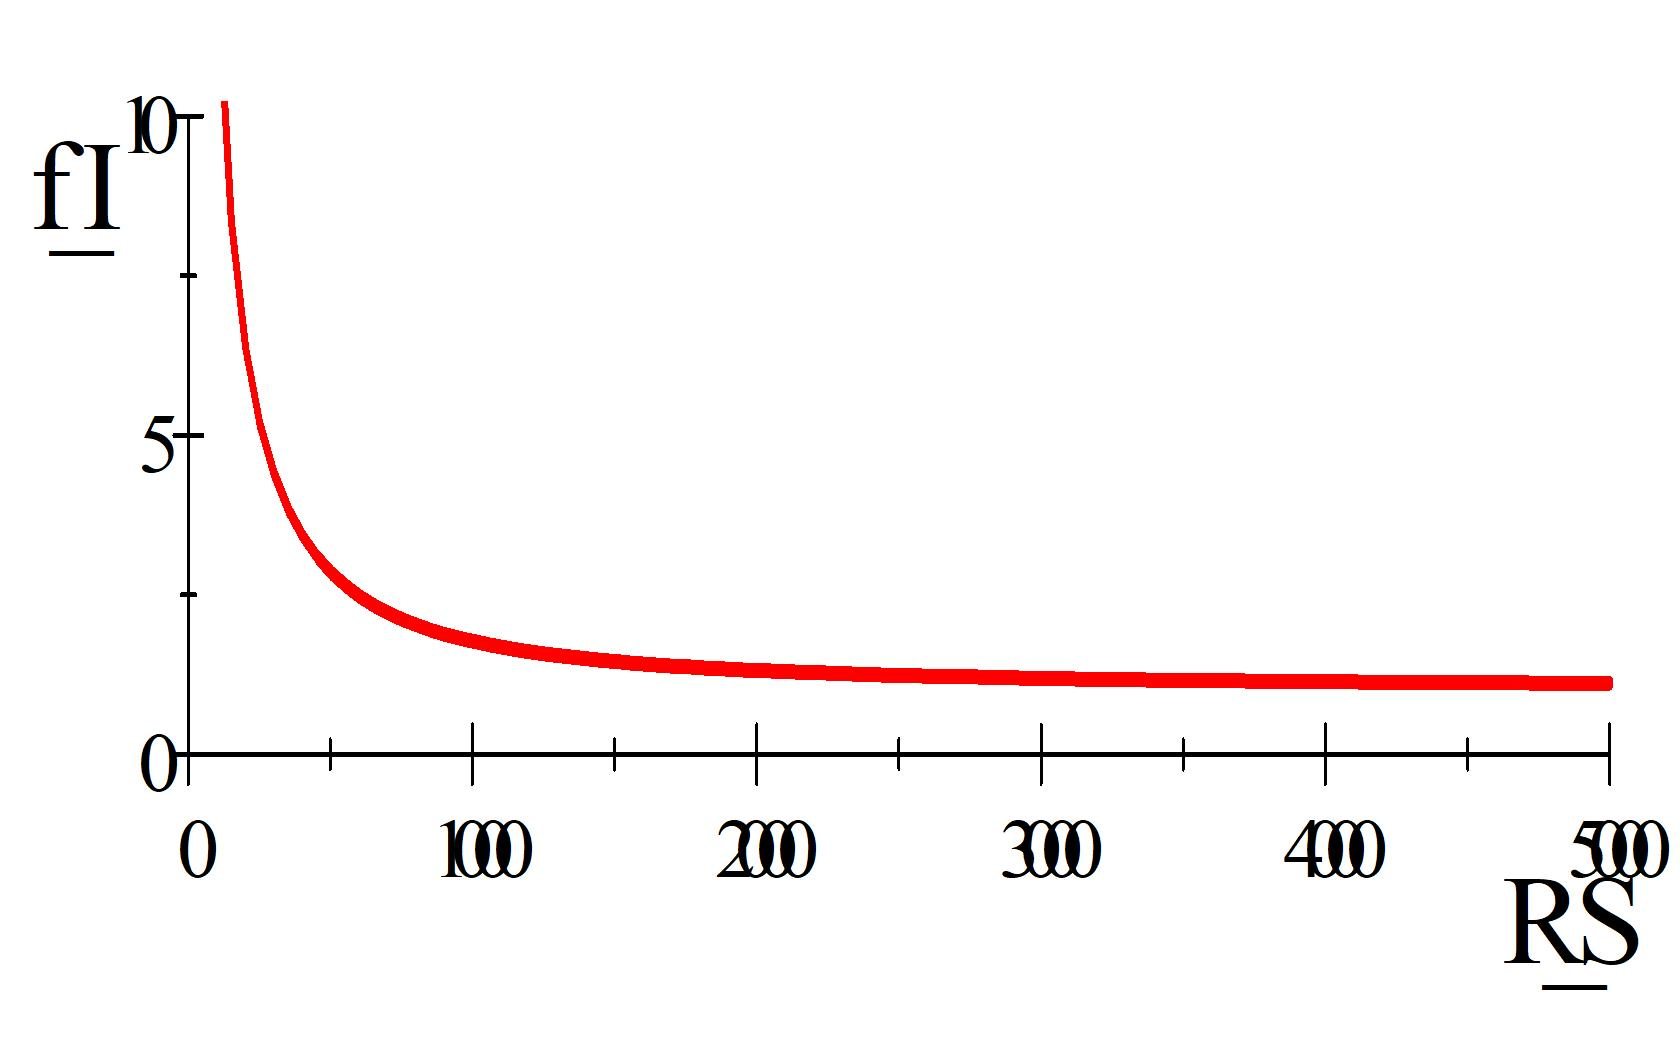
\includegraphics[width=4.5in,height=1.5in]{PH4CAV2V}
\end{figure}

Notice that after about $500\unit{\Omega}$ we are not going to get much of an improvement. So our choice of $R_{s}=500\unit{\Omega}$ seems good for this situation. Once you have a symbolic package or spreadsheet version of this calculation, picking different shunt resistors becomes fairly easy.

We should check, though. What did our $500\unit{\Omega}$ resistor do to our $\Delta V$ measurement? We found our current in the circuit to be 

\begin{equation*}
	I=3.\,\allowbreak 636\,4\times 10^{-4}\unit{A}
\end{equation*}

\noindent and our test resistor is $5000\unit{\Omega}$ so 

\begin{equation*}
	\Delta V_{test}=\left( 3.\,\allowbreak 636\,4\times 10^{-4}\unit{A}\right)\left( 5000\unit{\Omega}\right) =1.\,\allowbreak 818\,2\unit{V}
\end{equation*}

\noindent We know the power supply was providing $\Delta V_{ps}=2\unit{V}$. So we have introduced an error. We can find the percent difference 

\begin{equation*}
	\left( 100\right) \frac{1.\,\allowbreak 818\,2\unit{V}-2\unit{V}}{1.\,\allowbreak 818\,2\unit{V}}=-9.\,\allowbreak 998\,9\
\end{equation*}

\noindent which means the $\Delta V$ measurement will be $10\%$ low due to our inserting the shunt resistance. If we can live with a $10\%$ error, then we are fine. If not, it is back to iteration to find a better shunt resistance.

Of course, so far we have just found uncertainty in $\Delta V$ and $I$.
These are the uncertainties in our measuring devices that we built. Since
you are the manufacturer of these devices, you have had to calculate what
their uncertainties will be. When we design our own measuring devices, we
always have to do this. Of course you could have built the devices and then
watched the output to see where the digits fluctuate like we did with our
stand-alone multimeters. But the risk is that it might take a long time to
find a value for each part of our device that works together with the other
parts, and in the mean time we might burn up our equipment if we don't plan
for what we want first. You can check your uncertainty calculations by
looking at the fluctuation of the digits to see if we are right (or if some
other uncertainty factor has crept in that we haven't handled yet).

When we started this lab we said we were testing Ohm's law, and we wanted to find $R_{test}$ with it's uncertainty $\delta R_{test}$ to see if Ohm's law really
works. We can find $R_{test} = \frac{\Delta V}{I}$. But how do we find $\delta R_{test}$? In finding the uncertainty in our measuring devices we haven't found $\delta R_{test}.$ We could use standard error propagation again to do this. But let's not!  We will review a different way to find $\delta R_{test}.$

%%%%%%%%%%%%%%%%%%%%%%%%%%%%%%%%%%%%%%%%%%%%%%%%%%%%%%%%%%%%%%%%%%%%%%%
% Insert a linear fit module here. Your choices as of this writing are
%   a linear fit in excel 
%\input{Chapters/Module_Linear_fit_in_Excel.tex}
%   or a linear fit in python
\subsection{Using statistics to calculate uncertainty}

By now in a experimental design, I am usually at my tolerance limit for calculating uncertainties. You might ask, can't we get our powerful computers to help us out a little bit with finding the uncertainty? After all, we went to all the trouble to get the data on the computer. The answer is, yes!

Let's suppose we have done our experiment and we have some data that look like this: 

\begin{figure}[h!]
	\centering
	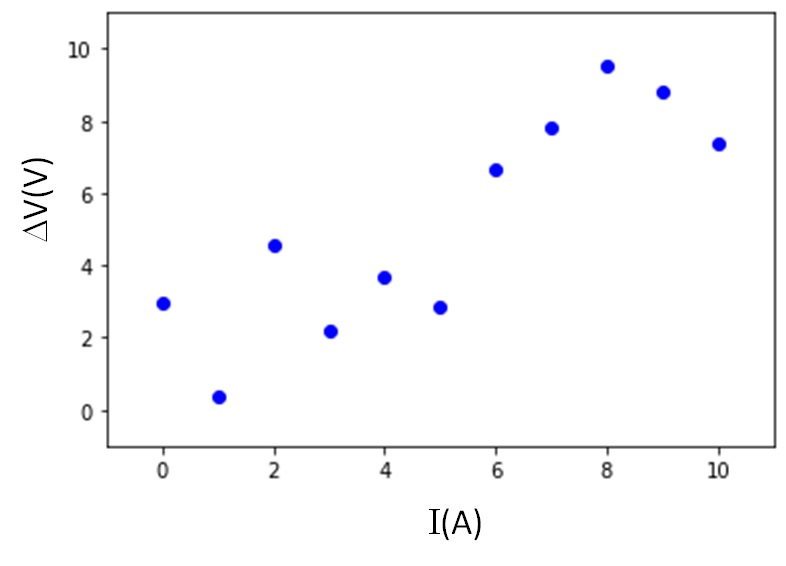
\includegraphics[width=3.563in,height=2.7345in]{linear_data}
\end{figure}

This looks pretty good. It seems to be sort of linear. We might guess from this that Ohm's law is begin obeyed.  We could calculate $R_{test}$ from each pair of $\Delta V$ and $I$ points and find it's uncertainty using standard error propagation. But it seems that it would be better to take all the points into our analysis to find $R_{test}.$ More data should give us a better estimate for $R_{test}.$  We want $R_{test},$ and $R_{test}$ is the slope of this line. So we could use this plot and it's slope to find $R_{test}$! We can use this! Back in PH150 you may have done such a thing using a \emph{curve fit}. In the next figure, a curve fit is shown for the data from the last figure. 

\begin{figure}[h!]
	\centering
	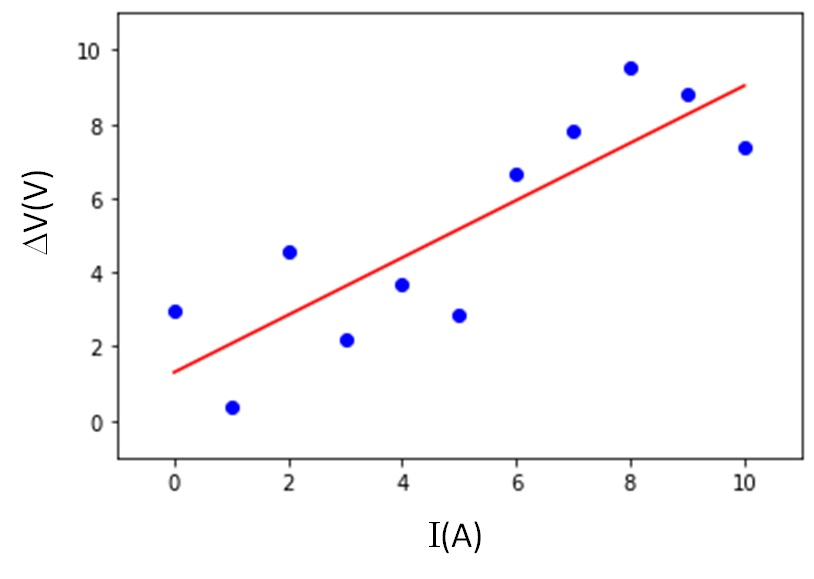
\includegraphics[width=3.563in,height=2.7345in]{linear_data_with_fit}
\end{figure}

Notice that I performed this curve fit in python, but if you are a not a great Python programer you could do this in Excel. You could also do this in LoggerPro or many other data analysis programs. If you need help finding a way to perform a curve fit, talk to your instructor. Here is an example code for doing the curve fit in python.

\vspace{0.24in}
\href{https://raw.githubusercontent.com/rtlines/IntermediateLabPH250/main/Code/linear_fit.py}{Download here}

\lstinputlisting[language=Arduino]{Code/linear_fit.py}

The scipy linregress() function uses the equation for a line 

\begin{equation*}
	y = result.slope*x + result.intercept
\end{equation*}

\noindent Our code gives the result

\begin {verbatim}
slope is   0.7737292152727273 +-  0.1612215125332822
intercept is   1.2996514309090914 +-  0.9537993308988922
program ended successfully
\end{verbatim}

\noindent which tells us that we have a slope of about $0.774.$ Since our graph
has $\Delta V$ on the vertical axis and $I$ on the horizontal axis we
recognize 
\begin{eqnarray*}
	\Delta V &=&R_{test}I+0 \\
           y &=&mx+b
\end{eqnarray*}

that $R_{test}$ must be the slope. We can see that the resistance for this example is about a tiny $0.774\unit{\Omega}$ because that is the slope of our fit line. But we know we need an uncertainty along with this nominal value. And low and behold! the scipy lineregress() function has already given us the data we need to find the errors on the slope and intercept as well! This was pretty easy!

Notice that in this analysis technique, we can often afford some error in our 
$\Delta V$ and $I$ values. So maybe a $9\%$ error (like we found in one of
our instrument designs) is not so bad. We may not have to work too hard to
get a wonderful choice of shunt resistor if we are going to use many data
points and the power of statistics to analyze the data in the end!

%%%%%%%%%%%%%%%%%%%%%%%%%%%%%%%%%%%%%%%%%%%%%%%%%%%%%%%%%%%%%%%%%%%%%%%

\subsection{Philosophical warning}

There was a lot to this reading. We talked about designing and building an
instrument. We used some physics, Ohm's law, in our design process. Then we
tested a physical model, Ohm's law, with our instrument. All these were good things, but maybe you wondered along the way if it is acceptable to test Ohm's law with an instrument that depends on Ohm's law. And the answer is a big NO!

This lab is practice, but it is imperfect practice. We do know that Ohm's
law works, so we are going to use it in designing instruments. But you
really need a different instrument, one that does not depend on Ohm's law,
to test Ohm's law in a credible way. In next week's lab, we will test a
different physical model with the same basic instrument that we built today. The instrument will depend on Ohm's law, but the new physical model must not if the experiment is to be valid.

%%%%%%%%%%%%%%%%%%%%%%%%%%%%%%%%%%%%%%%%%%%%%%%%%%%%%%%%%%%%%%%%%%%%%%%
% Normal semesters the proposal section goes here
%%%%%%%%%%%%%%%%%%%%%%%%%%%%%%%%%%%%%%%%%%%%%%%%%%%%%%%%%%%%%%%%%%%%%%%

\section{Proposals}

It's time to start thinking of what experiment you and your group will design. If you are taking PH250 as a block class we have to do this right at the start because it may take time to order in parts for your instrument that you will design. If you are taking PH250 as a full semester class, it is not as much of a hurry, but we still need lead time to order things. So even if it feels early, we need to think about this. You are required to write a proposal for this experiment. This is a document that is intended to persuade someone (your professor,  funding agency, yourself, etc.) that you should be given the resources and support to perform the experiment. The proposal consists of the following parts:

\begin{enumerate}
	\item Statement of the experimental problem
	
	\item Procedures and anticipated difficulties
	
	\item Proposed analysis and expected results
	
	\item Preliminary List of equipment needed
\end{enumerate}

\noindent Since you be writing each of these sections, let's discuss what should be in them.

\subsection{Statement of the experimental problem}

This is a physics class, so our experiment should be a physics experiment. The job of an experimental physicist is to test physics theory. So your statement of the experimental problem should include \textbf{what theory you are testing} and a brief, high level, overview of what you plan to do to test this theory.

\subsection{Procedures and anticipated difficulties}

Hopefully, your reader will be so excited by the thought of you testing your theory that he or she will want to know the details of what you plan to do. You should describe in some detail what you are planning. If there are hard parts of the procedure, tell how you plan to get through them.

\subsection{Proposed analysis and expected results}

You might think this is unfair. How are you supposed to know what analysis will be needed and what the results should be until you take the data? But really you both can, and should, make a good plan for your data analysis and figure out what your expected results should be. After all, you have a theory your are testing! You can encapsulate that theory into a predictive equation for your experiment. You can design your experimental apparatus, and put in the numbers from your experimental design. From this you can calculate what should be the outcome.

If you don't do this first, you don't know what equipment you will need or how sensitive that equipment needs to be. If you are trying to measure the size of your text book, an odometer that only measures in whole miles may not be the best choice of equipment. To know what you need, do the calculations in advance.

You should also do the error analysis. You will want to predict the uncertainty. A measurement of your laptop computer length that is good to $\pm 3\unit{m}$ is not very satisfying in most cases. Uncertainty in your result is governed by the uncertainty inherent in the measurements you will take. The uncertainty calculation tells you what sensitivity you will need in your measurement devices. Since you are choosing those measurement devices as part of your proposal, and you are choosing the inputs to your model equation (like the resistance and the capacitance in today's lab) you will know how much uncertainty they have, so you can do the calculation in advance.

You should do all of this symbolically if you can, numerically if you must, but almost never by hand (meaning don't use your calculator) giving single value results. Some measurements will come back poorer than you anticipated, or some piece of equipment will be unavailable. You don't want to have to redo all your calculations from scratch each time this happens. For example, in the event of an equipment problem, your analysis tells you if another piece of equipment is sufficiently sensitive, or if you need to find an exact replacement. When I perform an analysis like this, I try for a symbolic equation for uncertainty. I like to program these equations in Mathmatica, or Maple, or SAGE, or MathCAD, or whatever symbolic math processor I have. Alternately, you could code it into Python. Then, as actual measurements change, I instantly get new predictions. In the absence of a symbolic package, a spreadsheet program will do fine. A numerical program also is quick and easy to re-run with new numbers when no symbolic answer is found.

\subsection{Preliminary List of equipment needed}

Once you have done your analysis, you are ready to list the equipment you need and the sensitivity of the measurement equipment you need. Final approval of the project and the ultimate success of your experiment depend on the equipment you choose or are granted. You want to do a good job analyzing so you know what you need, and a good job describing the experiment so you are likely to have the equipment granted.

\subsection{Designing the Experiment}

Of course, as part of your proposal, you will have to design your experiment. In PH150 we learned that to design an experiment we needed the following steps. Some evidence of these steps should be found in your lab notebook:

\begin{enumerate}
	\item Identify the system to be examined. Identify the inputs and outputs. Describe your system in your lab notebook.
	
	\item Identify the model to be tested. Express the model in terms of an equation representing a prediction of the measurement you will make. Record this in your lab notebook.
	
	\item Plan how you will know if you are successful in your experiment. Plan graphs or other reporting devices. Record this in your lab notebook. This usually requires you to calculate the predicted uncertainty and to evaluate the relative size of the terms in the uncertainty equation (see below).
	
	\item Rectify your equation if needed. Record this in your lab notebook.
	
	\item Choose ranges of the variables. Record this in your lab notebook.
	
	\item Plan the experimental procedure. Record this in your lab notebook.
	
	\item Perform the experiment . Record this in your lab notebook (see next section).
\end{enumerate}

Let's just take a moment to recall what we learned from PH150 about group projects and lab notebooks.  You won't do all the work by yourself in a group project (we aren't in high school anymore!).  So you won't have an entry in your own lab notebook for everything that happens in your group project. For example, you might do the wiring, but someone else does the coding.  But if you say nothing about the coding, you have a huge hole in your record of what happened.  To solve this, you mention that the item happened (coding in our example) but just put in a reference to the person who did that part of the work.  So in our example you would put in a reference in your lab notebook to the lab notebook of the person who wrote the code.  That way, in your work group there is a clear path to what was done in everyone's lab notebooks.  This is what you do in real jobs!  So we will practice it here (and yes, it gets graded, because this isn't a real job, just a class).

\subsection{Using Uncertainty to refine experimental design.}

Suppose you plan to test our model for resistance from your PH220 text book. The equation for resistance is 

\begin{equation*}
	R=\rho \frac{\ell }{A}
\end{equation*}

\noindent where $\rho $ is the resistivity, the material properties of the material that makes wire or resistor have friction. The length of the wire or resistor is $\ell $, and $A$ is the cross sectional area. We could find the uncertainty in $R$

\begin{equation*}
	\delta R=\sqrt{\left( \frac{\partial R}{\partial \rho }\delta \rho \right)
		^{2}+\left( \frac{\partial R}{\partial \ell }\delta \ell \right) ^{2}+\left( 
		\frac{\partial R}{\partial A}\delta A\right) ^{2}}
\end{equation*}

\noindent The first term in the square root is 

\begin{equation*}
	\left( \frac{\partial R}{\partial \rho }\delta \rho \right) ^{2}=\left( 
	\frac{\ell }{A}\delta \rho \right) ^{2}
\end{equation*}

\noindent and the other two terms are 

\begin{equation*}
	\left( \frac{\partial R}{\partial \ell }\delta \ell \right) ^{2}=\left( 
	\frac{\rho }{A}\delta \ell \right) ^{2}
\end{equation*}

\begin{equation*}
	\left( \frac{\partial R}{\partial A}\delta A\right) ^{2}=\left( -\rho \frac{%
		\ell }{A^{2}}\delta A\right) ^{2}
\end{equation*}

And suppose that our design is to have a copper wire with 

\begin{eqnarray*}
	\rho &=&1.68\pm 0.03\times 10^{-8}\unit{\Omega}\unit{m} \\
	\ell &=&5.0\pm 0.1\unit{m} \\
	A &=&5.0\times 10^{-10}\unit{m}^{2}\unit{m}^{2}
\end{eqnarray*}

\noindent This would give a resistance of 

\begin{eqnarray*}
	R_{new} &=&1.68\times 10^{-8}\unit{\Omega}\unit{m}\frac{5\unit{m}}{5.0\times 10^{-10}\unit{m}^{2}} \\
	&=&168.0\unit{\Omega}
\end{eqnarray*}

We can calculate each of our terms from the $\delta R$ equation. 

\begin{equation*}
	\left( \frac{\ell }{A}\delta \rho \right) ^{2}=\left( \frac{5\unit{m}}{%
		5.0\times 10^{-10}\unit{m}^{2}}\left( 0.03\times 10^{-8}\unit{\Omega	}\unit{m}\right) \right) ^{2}=9.0\unit{\Omega}^{2}
\end{equation*}

\begin{equation*}
	\left( \frac{\rho }{A}\delta \ell \right) ^{2}=\left( \frac{1.68\times
		10^{-8}\unit{\Omega}\unit{m}}{5.0\times 10^{-10}\unit{m}^{2}}\left( 0.1\unit{m}\right) \right) 	^{2}=11.\,\allowbreak 290\unit{\Omega}^{2}
\end{equation*}

\begin{equation*}
	\left( -\rho \frac{\ell }{A^{2}}\delta A\right) ^{2}=\left( -\left(
	1.68\times 10^{-8}\unit{\Omega}\unit{m}\right) \frac{\left( 5\unit{m}\right) }{\left( 5.0\times 10^{-10} \unit{m}^{2}\right) ^{2}}\left( 0.1\times 10^{-9}\unit{m}^{2}\right) \right)
	^{2}=1129.\,\allowbreak 0\unit{\Omega}^{2}
\end{equation*}

\noindent The overall uncertainty then would be

\begin{equation*}
	\delta R=\sqrt{9.0\unit{\Omega}^{2}+11.\,\allowbreak 290\unit{\Omega}^{2}+1129.\,\allowbreak 0\unit{\Omega}^{2}}=33.\,\allowbreak 901\unit{\Omega}
\end{equation*}

So with this design we predict a fractional uncertainty of 

\begin{equation*}
	\frac{33.\,\allowbreak 901\unit{\Omega}}{168.0\unit{\Omega}}=0.201\,79
\end{equation*}

or a little over $20\%.$ This is not a great design. We would like a much lower uncertainty, something that gives a fractional uncertainty more like $1\%.$ It is clear that the last term has the highest contribution to the uncertainty, so this is the term that needs fixing. One method of fixing the problem would be to decrease $A.$ We could try $1.0\pm 0.1\times 10^{-9}\unit{m}^{2}.$ In order to have the same resistance we will also have to change the length of the wire from $10\unit{m}$ to $5\unit{m}$. 

\begin{eqnarray*}
	\rho &=&1.68\pm 0.03\times 10^{-8}\unit{\Omega}\unit{m} \\
	\ell &=&10.0\pm 0.1\unit{m} \\
	A &=&1.0\pm 0.1\times 10^{-9}\unit{m}^{2}
\end{eqnarray*}

Checking we see we do get the same resistance 

\begin{eqnarray*}
	R &=&1.68\times 10^{-8}\unit{\Omega	}\unit{m}\frac{10\unit{m}}{1.0\times 10^{-9}\unit{m}^{2}} \\
	&=&168\unit{\Omega}
\end{eqnarray*}

\noindent But now for the last term we would get 

\begin{equation*}
	\left( -\rho \frac{\ell }{A^{2}}\delta A\right) ^{2}=\left( -\left(
	1.68\times 10^{-8}\unit{\Omega}\unit{m}\right) \frac{\left( 10\unit{m}\right) }{\left( 1.0\times 10^{-9}\unit{m}^{2}\right) ^{2}}\left( 0.1\times 10^{-9}\unit{m}^{2}\right) \right)^{2}=282.\,\allowbreak 24\unit{\Omega}^{2}
\end{equation*}

\noindent which is better. But we have to check to make sure our design change didn't
cause a large rise in the other two terms. 

\begin{equation*}
	\left( \frac{\ell }{A}\delta \rho \right) ^{2}=\left( \frac{10\unit{m}}{		1.0\times 10^{-9}\unit{m}^{2}}\left( 0.03\times 10^{-8}\unit{\Omega}\unit{m}\right) \right) ^{2}=9.0\unit{\Omega}^{2}
\end{equation*}

\begin{equation*}
	\left( \frac{\rho }{A}\delta \ell \right) ^{2}=\left( \frac{1.68\times
		10^{-8}\unit{\Omega}\unit{m}}{1.0\times 10^{-9}\unit{m}^{2}}\left( 0.1\unit{m}\right) \right)^{2}=2.8224\unit{\Omega}^{2}
\end{equation*}

The first term was hurt by our new design change, but not badly. So with the new design the overall uncertainty would be 

\begin{equation*}
	\delta R=\sqrt{9.0\unit{\Omega}^{2}+2.8224\unit{\Omega}^{2}+282.\,\allowbreak 24\unit{\Omega		}^{2}}=17.\,\allowbreak 148\unit{\Omega}
\end{equation*}

\noindent So with this new design we predict a fractional uncertainty of

\begin{equation*}
	\frac{17.\,\allowbreak 148\unit{\Omega}}{168.0\unit{\Omega	}}=0.102\,07
\end{equation*}

which is about $\allowbreak 10.\%.$ This is much better. From our uncertainty terms, we can see that to do better we need to improve both the $\delta A$ term and the $\delta \ell $ terms because they are now about the same size. Probably no one in our class is really testing the resistance equation. This is just an example. But the point we need to take away from this example is that \textbf{the terms in our uncertainty calculation tell us how to modify our experimental design.}

There is a refinement we could make to our process. really there are no area measurement devices available, so what we would do is measure the diameter of the wire and calculate the area.

\begin{equation*}
	A=\frac{1}{4}\pi D^{2}
\end{equation*}

We could find $\delta A$ by using our propagation of uncertainty equation again, or we could modify our resistance equation so that it is in terms of what we actually measure.

\begin{equation*}
	R=\rho \frac{4\ell }{\pi D^{2}}
\end{equation*}

\noindent and calculate our uncertainty in terms of $\rho ,$ $\ell ,$ and $D.$ That is preferred and usually less work. The general rule is to express your model equation in terms of what you will actually measure before you calculate the uncertainty terms.

The moral of this long story is that we must calculate the uncertainty \textbf{ \emph{as part of the design process} }. It is probably best to use a symbolic math processor or at lease a python program or spreadsheet so that as the design changes your uncertainty estimate will change too without having to manually recalculate it.




\section{Lab Assignment}

\begin{enumerate}
\item Build the instrument

\begin{enumerate}
\item Choose a test resistor in the $1\unit{k\Omega}$ to $10\unit{k\Omega}$ range and a shunt resistor. You will have to check your values using the math we discussed above to make sure they will work. If your first shunt resistor choice works, use it. If not, iterate until you have a shunt resistance that will work.

	\item Modify your voltmeter sketch to measure both the voltage and the current. (Check the voltage, currents, and their uncertainties with the serial monitor to make sure things seem good).

	\item Build your voltmeter and ammeter so your Arduino is taking $\left(I,\Delta V\right) $ pares and reporting them. Reporting to the serial monitor is fine for a start. 
	\begin{figure}[h!]
		\centering
		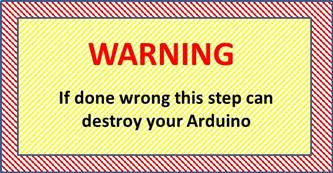
\includegraphics[width=1.8507in,height=0.9677in]{PH4CAW36}
	\end{figure}
	\noindent if you based your sketch on the simple voltmeter, make sure you don't use voltages outside the $0\unit{V}$ to $+5\unit{V}$ range! Include expected uncertainties for your $\Delta V$ and $I$ measurements.

	\item Check your lab group's instruments to see if they work, and have your lab group members check yours.
\end{enumerate}

\item Test Ohm's law

\begin{enumerate}
	\item Take 10-15 measurements of $\Delta V$ and $I.$ For each $\Delta V$ measurement change the $\Delta V$ setting on the power supply a small amount (don't go over $5\unit{V}$ if you are using the simple voltmeter!).
	
	\item Plot voltage vs. current and fit a curve to the data.

	\item Determine the resistance from this curve fit and its uncertainty.

	\item Finally, determine if your results support the Ohm model for how potential and current are related?

	\item Compare your data and conclusions to the data and conclusions of your lab group members. Have them look at your results as well.
\end{enumerate}

	\item Using the same new instrument, repeat part 2 for a diode by replacing your test resistance with the diode. Do your results support the Ohm model for how potential and current are related?

	\item Could you have your Arduino sketch report the calculated uncertainties for $\Delta V,$ $I,$ and $R?$ If you have time (you probably won't) give this a try.
\end{enumerate}


\vfill

